% vim: set tabstop=4 :
%**********************************************************
\chapter{人流シミュレーション}
%\chapter{本来なら問題定義や背景的な何かを書く}
\label{sec:background}
%**********************************************************
人流シミュレーションは,コンピュータ上で人の動きを再現する手法であり,
図\ref{fig:aaaa}に人流シミュレーションの例を示す.図\ref{fig:aaaa}中の
青色の丸は右側に進む人,緑色の丸は左側に進む人,黄色の四角は壁,青色の四角
は障害物である.
赤色の障害物は,自動販売機やゴミ箱などの移動が可能である設置物である.
図\ref{fig:aaaa}の例では,通路が赤色の障害物によって通路が狭くなっている
ため,人の滞留や混雑が起きているため,赤色の障害物を撤去することで滞留や
混雑を防ぐことができる.
図\ref{fig:aaaa}のような混雑や滞留を発見するためには,実際に多くの人で
実験する必要があるため,時間や費用がかかる.一方で,
人流シミュレーションは,コンピュータ上で再現できることから
,実際に多くの人を用いて実験するよりも,必要な時間や金額を抑えることが可能である.
このように,人流シミュレーションの目的は,人の滞留や混雑が起きないように
対策することである.
このため,人流シミュレーションは,大規模なイベントを企画する企業や
大規模や施設を設計,建築する建設業などで活用されている(参考文献).
人流シミュレーションを活用することで,事前に人の流れを予測することが可能に
なり,地震や火災などの有事のときに,非常灯や看板の配置,警備員の配置などを
最適化できるため,適切な誘導が行うことが可能になる.
%人流シミュレーションに必要な要素
人流シミュレーションを用いて解析するためには,空間を再現するための
空間のモデル化,歩行者を再現するための歩行者のモデル化,障害物や壁を再現
するための障害物のモデル化が必要である.

\begin{figure}[h]
    \begin{center}
     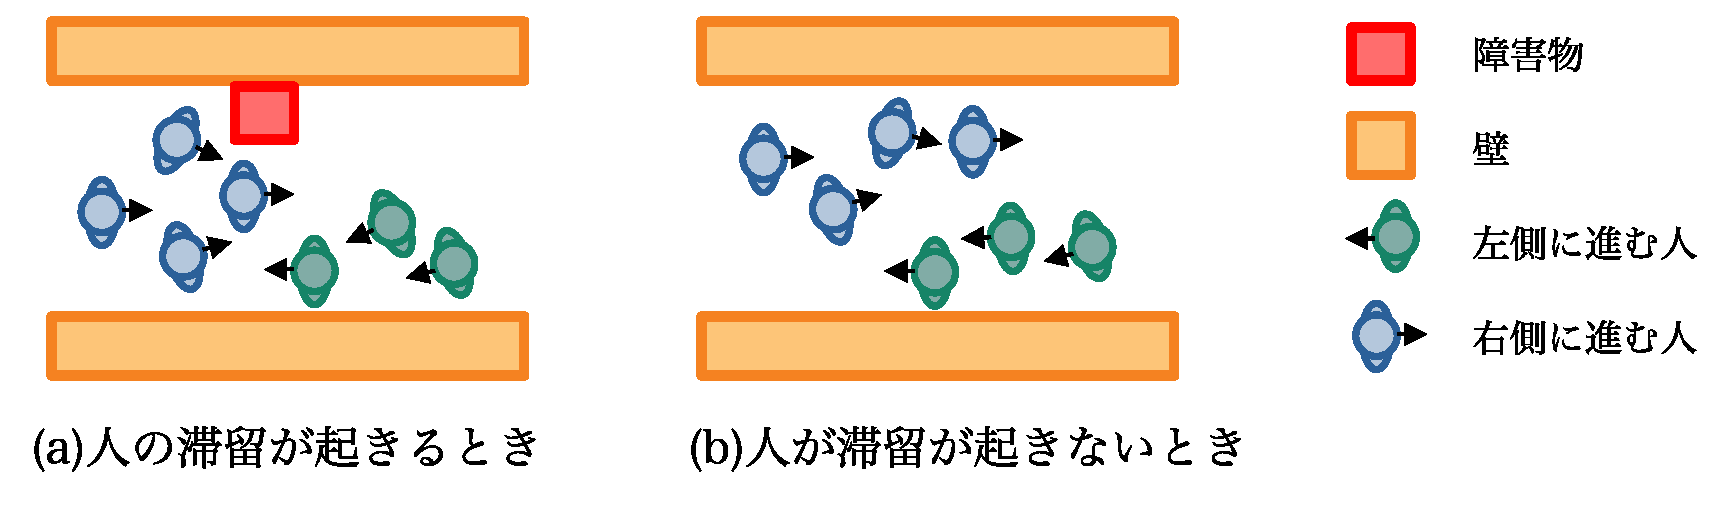
\includegraphics[width=14cm,clip]{figure/jinryu_image2_r2.eps}
     \caption{人流シミュレーションの活用例}
     \label{fig:jinryu_image2}
    \end{center}
\end{figure}


\section{空間モデル}
空間モデルは,解析したい場所をコンピュータで計算するために,空間を離散化するための
ものである.
シミュレーション対象が海岸から近い都市や人口が多い都市などの道路上の人々の流れを解析するためには,
数千人から数万人の解析が可能なネットワークモデルが用いられる(参考文献).
また,シミュレーション対象が商業施設や駅構内などの施設上の人々を解析するためには,
フロアフィールドモデルや連続座標モデルが用いられる(参考文献).



\subsection{ネットワークモデル}
ネットワークモデルは,

\begin{figure}[h]
    \begin{center}
     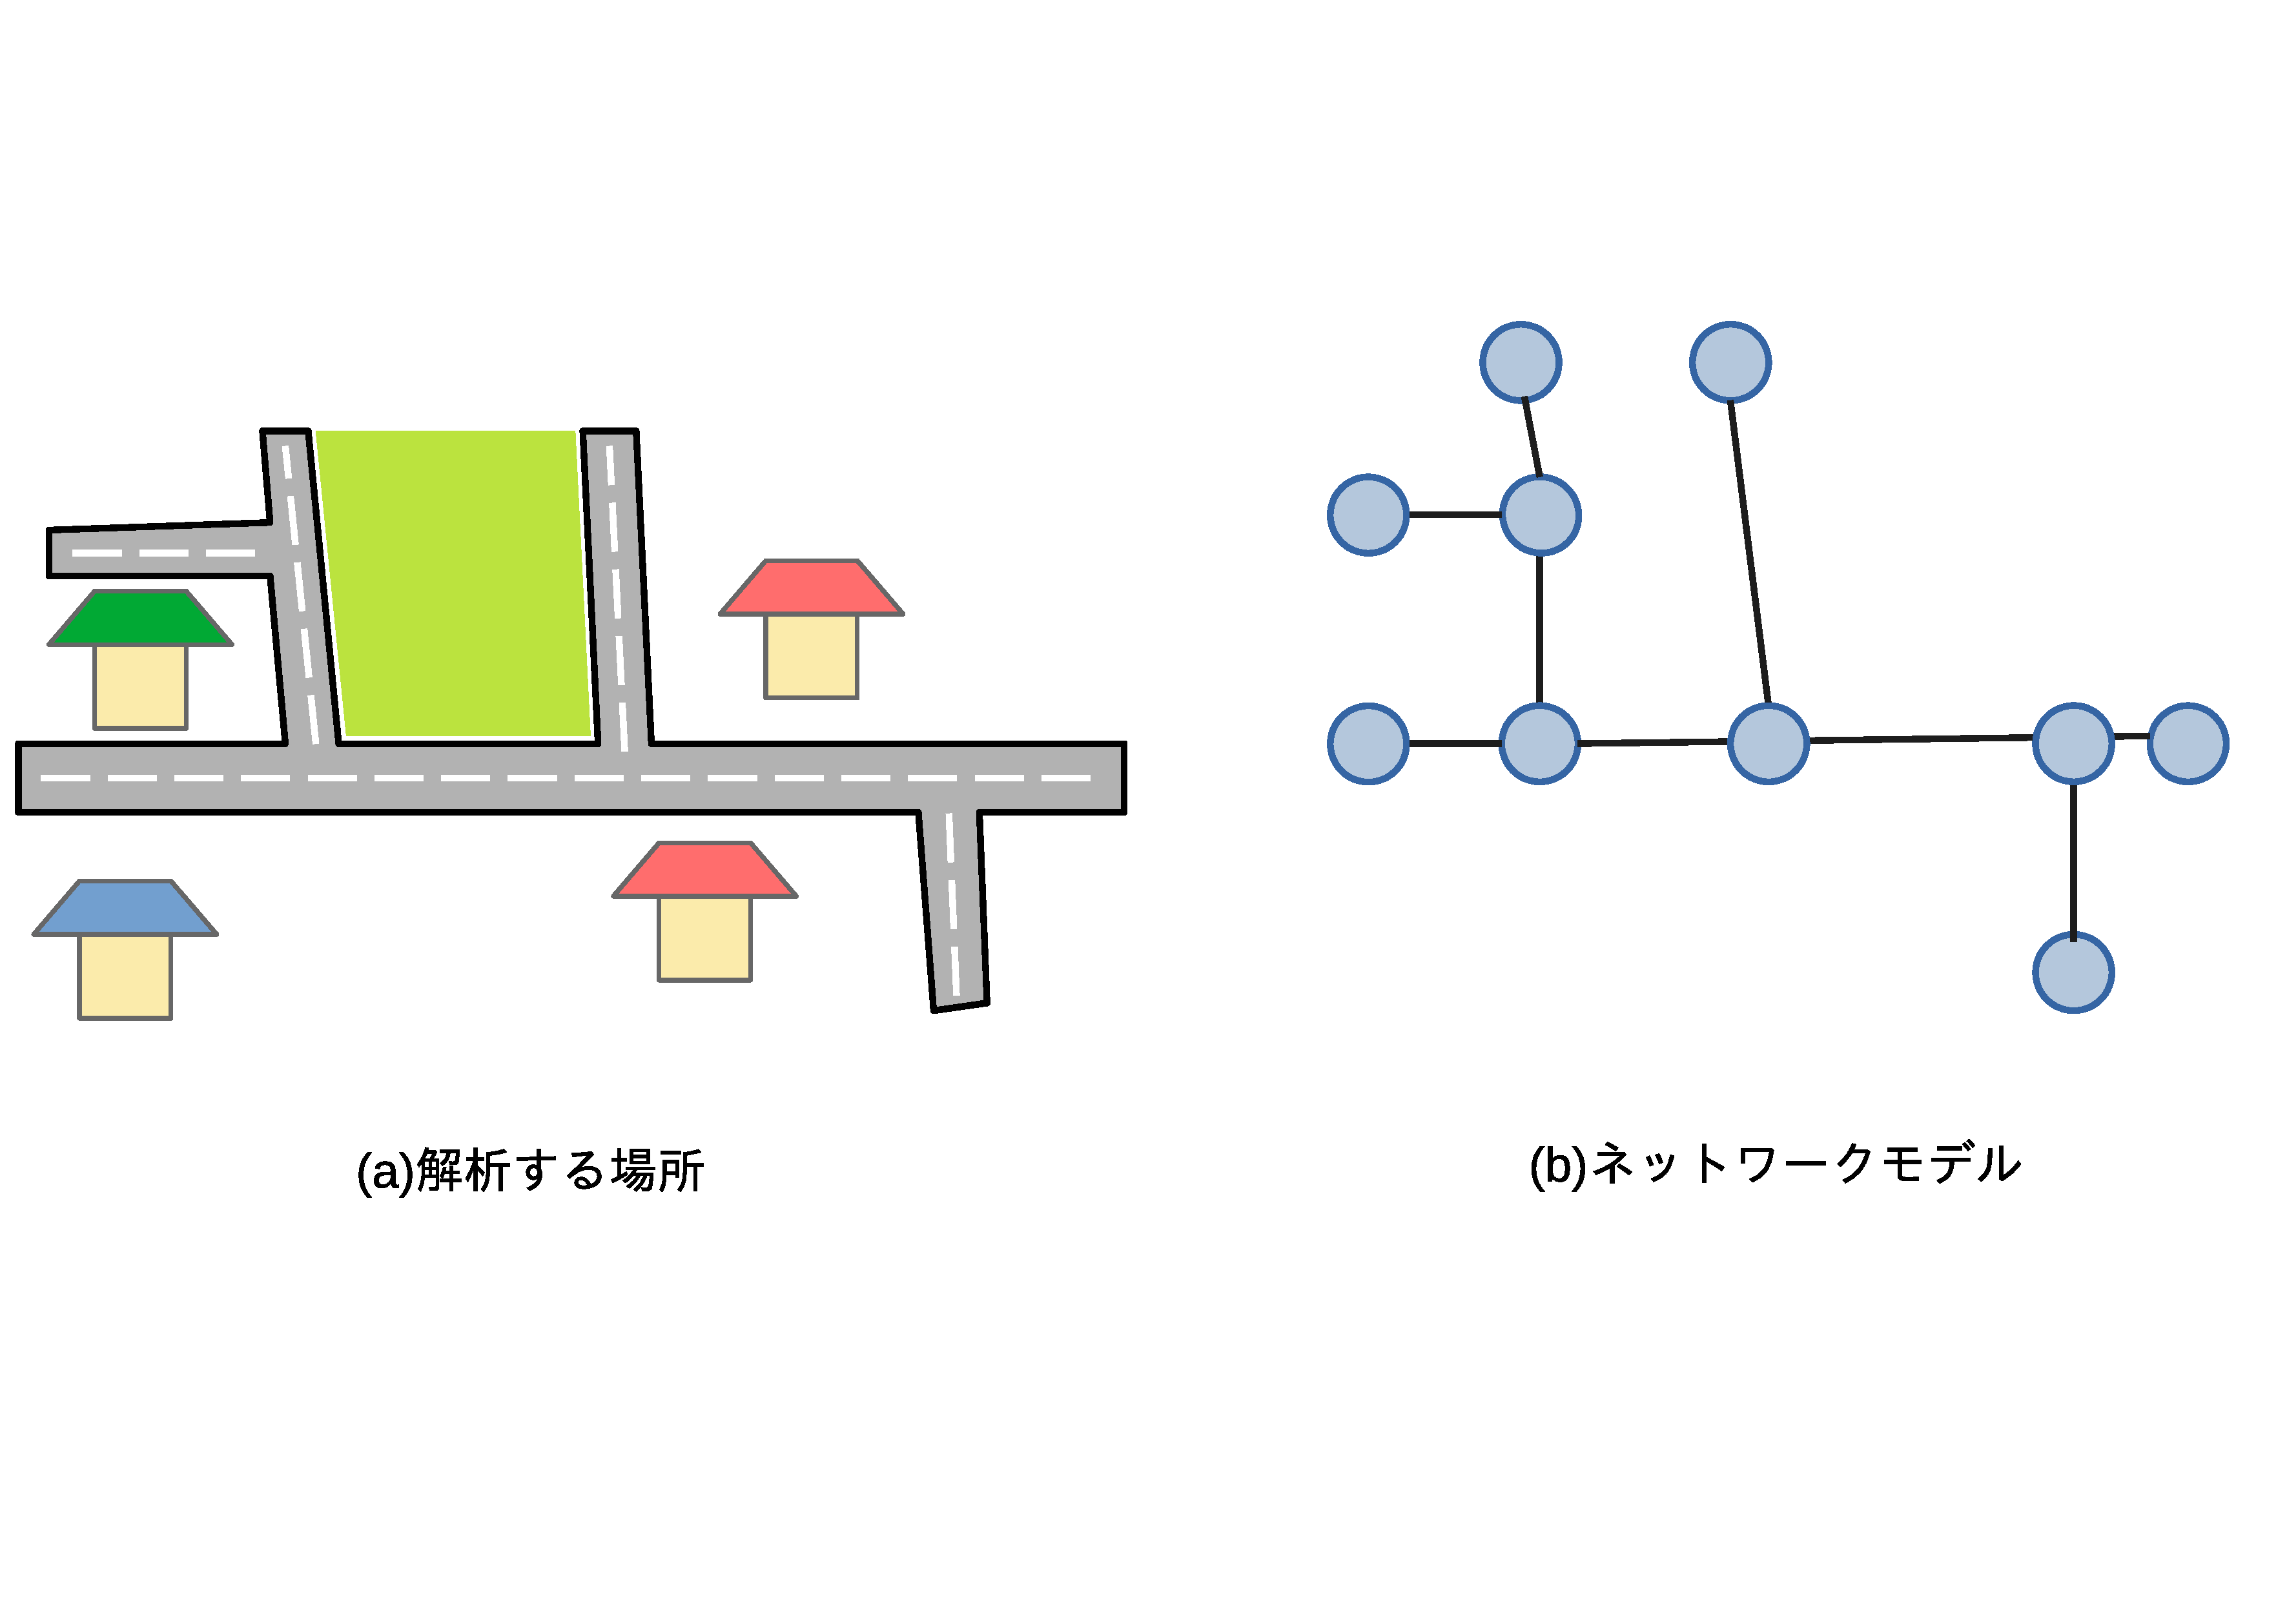
\includegraphics[width=14cm,clip]{figure/networkmodel_ex.eps}
     \caption{ネットワークモデルの例}
     \label{fig:jinryu_image2}
    \end{center}
\end{figure}


\subsection{フロアフィールドモデル}
フロアフィールドモデルは,

\subsection{連続座標モデル}
連続座標モデルは,

\section{歩行者モデル}

\subsection{セルオートマトン}

\subsection{RVOモデル}

\subsection{ソーシャルフォースモデル}

\section{障害物モデル}

\subsection{粒子によるモデル化}

\subsection{矩形によるモデル化}

\section{経路の設定}

\subsection{ダイクストラ法}



%1ブロックが10×30文字です
ああああああああああああああああああああああああああああああ
ああああああああああああああああああああああああああああああ
ああああああああああああああああああああああああああああああ
ああああああああああああああああああああああああああああああ
ああああああああああああああああああああああああああああああ
ああああああああああああああああああああああああああああああ
ああああああああああああああああああああああああああああああ
ああああああああああああああああああああああああああああああ
ああああああああああああああああああああああああああああああ
ああああああああああああああああああああああああああああああ
%
ああああああああああああああああああああああああああああああ
ああああああああああああああああああああああああああああああ
ああああああああああああああああああああああああああああああ
ああああああああああああああああああああああああああああああ
ああああああああああああああああああああああああああああああ
ああああああああああああああああああああああああああああああ
ああああああああああああああああああああああああああああああ
ああああああああああああああああああああああああああああああ
ああああああああああああああああああああああああああああああ
ああああああああああああああああああああああああああああああ
%
Penguin
ああああああああああああああああああああああああああああああ
ああああああああああああああああああああああああああああああ
ああああああああああああああああああああああああああああああ
ああああああああああああああああああああああああああああああ
ああああああああああああああああああああああああああああああ
ああああああああああああああああああああああああああああああ
ああああああああああああああああああああああああああああああ
ああああああああああああああああああああああああああああああ
ああああああああああああああああああああああああああああああ
ああああああああああああああああああああああああああああああ
%
ああああああああああああああああああああああああああああああ
ああああああああああああああああああああああああああああああ
ああああああああああああああああああああああああああああああ
ああああああああああああああああああああああああああああああ
ああああああああああああああああああああああああああああああ
ああああああああああああああああああああああああああああああ
ああああああああああああああああああああああああああああああ
ああああああああああああああああああああああああああああああ
ああああああああああああああああああああああああああああああ
ああああああああああああああああああああああああああああああ
%
ああああああああああああああああああああああああああああああ
ああああああああああああああああああああああああああああああ
ああああああああああああああああああああああああああああああ
ああああああああああああああああああああああああああああああ
ああああああああああああああああああああああああああああああ
ああああああああああああああああああああああああああああああ
ああああああああああああああああああああああああああああああ
ああああああああああああああああああああああああああああああ
ああああああああああああああああああああああああああああああ
ああああああああああああああああああああああああああああああ
ああああああああああああああああああああああああああああああ
%
ああああああああああああああああああああああああああああああ
ああああああああああああああああああああああああああああああ
ああああああああああああああああああああああああああああああ
ああああああああああああああああああああああああああああああ
ああああああああああああああああああああああああああああああ
ああああああああああああああああああああああああああああああ
ああああああああああああああああああああああああああああああ
ああああああああああああああああああああああああああああああ
ああああああああああああああああああああああああああああああ
%
ああああああああああああああああああああああああああああああ
ああああああああああああああああああああああああああああああ
ああああああああああああああああああああああああああああああ
ああああああああああああああああああああああああああああああ
ああああああああああああああああああああああああああああああ
ああああああああああああああああああああああああああああああ
ああああああああああああああああああああああああああああああ
ああああああああああああああああああああああああああああああ
ああああああああああああああああああああああああああああああ
ああああああああああああああああああああああああああああああ
%
ああああああああああああああああああああああああああああああ
ああああああああああああああああああああああああああああああ
ああああああああああああああああああああああああああああああ
ああああああああああああああああああああああああああああああ
ああああああああああああああああああああああああああああああ
あああああああああああああああああああああ
あああああああああああああああああああああ
%
%\chapter{背景(1671文字)}

%***** END ************************************************
